%% bare_jrnl.tex
%% V1.4b
%% 2015/08/26
%% by Michael Shell
%% see http://www.michaelshell.org/
%% for current contact information.
%%
%% This is a skeleton file demonstrating the use of IEEEtran.cls
%% (requires IEEEtran.cls version 1.8b or later) with an IEEE
%% journal paper.
%%
%% Support sites:
%% http://www.michaelshell.org/tex/ieeetran/
%% http://www.ctan.org/pkg/ieeetran
%% and
%% http://www.ieee.org/

%%*************************************************************************
%% Legal Notice:
%% This code is offered as-is without any warranty either expressed or
%% implied; without even the implied warranty of MERCHANTABILITY or
%% FITNESS FOR A PARTICULAR PURPOSE! 
%% User assumes all risk.
%% In no event shall the IEEE or any contributor to this code be liable for
%% any damages or losses, including, but not limited to, incidental,
%% consequential, or any other damages, resulting from the use or misuse
%% of any information contained here.
%%
%% All comments are the opinions of their respective authors and are not
%% necessarily endorsed by the IEEE.
%%
%% This work is distributed under the LaTeX Project Public License (LPPL)
%% ( http://www.latex-project.org/ ) version 1.3, and may be freely used,
%% distributed and modified. A copy of the LPPL, version 1.3, is included
%% in the base LaTeX documentation of all distributions of LaTeX released
%% 2003/12/01 or later.
%% Retain all contribution notices and credits.
%% ** Modified files should be clearly indicated as such, including  **
%% ** renaming them and changing author support contact information. **
%%*************************************************************************


% *** Authors should verify (and, if needed, correct) their LaTeX system  ***
% *** with the testflow diagnostic prior to trusting their LaTeX platform ***
% *** with production work. The IEEE's font choices and paper sizes can   ***
% *** trigger bugs that do not appear when using other class files.       ***                          ***
% The testflow support page is at:
% http://www.michaelshell.org/tex/testflow/



\documentclass[journal]{IEEEtran}
\usepackage{graphicx}
%
% If IEEEtran.cls has not been installed into the LaTeX system files,
% manually specify the path to it like:
% \documentclass[journal]{../sty/IEEEtran}





% Some very useful LaTeX packages include:
% (uncomment the ones you want to load)


% *** MISC UTILITY PACKAGES ***
%
%\usepackage{ifpdf}
% Heiko Oberdiek's ifpdf.sty is very useful if you need conditional
% compilation based on whether the output is pdf or dvi.
% usage:
% \ifpdf
%   % pdf code
% \else
%   % dvi code
% \fi
% The latest version of ifpdf.sty can be obtained from:
% http://www.ctan.org/pkg/ifpdf
% Also, note that IEEEtran.cls V1.7 and later provides a builtin
% \ifCLASSINFOpdf conditional that works the same way.
% When switching from latex to pdflatex and vice-versa, the compiler may
% have to be run twice to clear warning/error messages.






% *** CITATION PACKAGES ***
%
%\usepackage{cite}
% cite.sty was written by Donald Arseneau
% V1.6 and later of IEEEtran pre-defines the format of the cite.sty package
% \cite{} output to follow that of the IEEE. Loading the cite package will
% result in citation numbers being automatically sorted and properly
% "compressed/ranged". e.g., [1], [9], [2], [7], [5], [6] without using
% cite.sty will become [1], [2], [5]--[7], [9] using cite.sty. cite.sty's
% \cite will automatically add leading space, if needed. Use cite.sty's
% noadjust option (cite.sty V3.8 and later) if you want to turn this off
% such as if a citation ever needs to be enclosed in parenthesis.
% cite.sty is already installed on most LaTeX systems. Be sure and use
% version 5.0 (2009-03-20) and later if using hyperref.sty.
% The latest version can be obtained at:
% http://www.ctan.org/pkg/cite
% The documentation is contained in the cite.sty file itself.






% *** GRAPHICS RELATED PACKAGES ***
%
\ifCLASSINFOpdf
  % \usepackage[pdftex]{graphicx}
  % declare the path(s) where your graphic files are
  % \graphicspath{{../pdf/}{../jpeg/}}
  % and their extensions so you won't have to specify these with
  % every instance of \includegraphics
  % \DeclareGraphicsExtensions{.pdf,.jpeg,.png}
\else
  % or other class option (dvipsone, dvipdf, if not using dvips). graphicx
  % will default to the driver specified in the system graphics.cfg if no
  % driver is specified.
  % \usepackage[dvips]{graphicx}
  % declare the path(s) where your graphic files are
  % \graphicspath{{../eps/}} 
  % and their extensions so you won't have to specify these with
  % every instance of \includegraphics
  % \DeclareGraphicsExtensions{.eps}
\fi
% graphicx was written by David Carlisle and Sebastian Rahtz. It is
% required if you want graphics, photos, etc. graphicx.sty is already
% installed on most LaTeX systems. The latest version and documentation
% can be obtained at: 
% http://www.ctan.org/pkg/graphicx
% Another good source of documentation is "Using Imported Graphics in
% LaTeX2e" by Keith Reckdahl which can be found at:
% http://www.ctan.org/pkg/epslatex
%
% latex, and pdflatex in dvi mode, support graphics in encapsulated
% postscript (.eps) format. pdflatex in pdf mode supports graphics
% in .pdf, .jpeg, .png and .mps (metapost) formats. Users should ensure
% that all non-photo figures use a vector format (.eps, .pdf, .mps) and
% not a bitmapped formats (.jpeg, .png). The IEEE frowns on bitmapped formats
% which can result in "jaggedy"/blurry rendering of lines and letters as
% well as large increases in file sizes.
%
% You can find documentation about the pdfTeX application at:
% http://www.tug.org/applications/pdftex





% *** MATH PACKAGES ***
%
%\usepackage{amsmath}
% A popular package from the American Mathematical Society that provides
% many useful and powerful commands for dealing with mathematics.
%
% Note that the amsmath package sets \interdisplaylinepenalty to 10000
% thus preventing page breaks from occurring within multiline equations. Use:
%\interdisplaylinepenalty=2500
% after loading amsmath to restore such page breaks as IEEEtran.cls normally
% does. amsmath.sty is already installed on most LaTeX systems. The latest
% version and documentation can be obtained at:
% http://www.ctan.org/pkg/amsmath





% *** SPECIALIZED LIST PACKAGES ***
%
%\usepackage{algorithmic}
% algorithmic.sty was written by Peter Williams and Rogerio Brito.
% This package provides an algorithmic environment fo describing algorithms.
% You can use the algorithmic environment in-text or within a figure
% environment to provide for a floating algorithm. Do NOT use the algorithm
% floating environment provided by algorithm.sty (by the same authors) or
% algorithm2e.sty (by Christophe Fiorio) as the IEEE does not use dedicated
% algorithm float types and packages that provide these will not provide
% correct IEEE style captions. The latest version and documentation of
% algorithmic.sty can be obtained at:
% http://www.ctan.org/pkg/algorithms
% Also of interest may be the (relatively newer and more customizable)
% algorithmicx.sty package by Szasz Janos:
% http://www.ctan.org/pkg/algorithmicx




% *** ALIGNMENT PACKAGES ***
%
%\usepackage{array}
% Frank Mittelbach's and David Carlisle's array.sty patches and improves
% the standard LaTeX2e array and tabular environments to provide better
% appearance and additional user controls. As the default LaTeX2e table
% generation code is lacking to the point of almost being broken with
% respect to the quality of the end results, all users are strongly
% advised to use an enhanced (at the very least that provided by array.sty)
% set of table tools. array.sty is already installed on most systems. The
% latest version and documentation can be obtained at:
% http://www.ctan.org/pkg/array


% IEEEtran contains the IEEEeqnarray family of commands that can be used to
% generate multiline equations as well as matrices, tables, etc., of high
% quality.




% *** SUBFIGURE PACKAGES ***
%\ifCLASSOPTIONcompsoc
%  \usepackage[caption=false,font=normalsize,labelfont=sf,textfont=sf]{subfig}
%\else
%  \usepackage[caption=false,font=footnotesize]{subfig}
%\fi
% subfig.sty, written by Steven Douglas Cochran, is the modern replacement
% for subfigure.sty, the latter of which is no longer maintained and is
% incompatible with some LaTeX packages including fixltx2e. However,
% subfig.sty requires and automatically loads Axel Sommerfeldt's caption.sty
% which will override IEEEtran.cls' handling of captions and this will result
% in non-IEEE style figure/table captions. To prevent this problem, be sure
% and invoke subfig.sty's "caption=false" package option (available since
% subfig.sty version 1.3, 2005/06/28) as this is will preserve IEEEtran.cls
% handling of captions.
% Note that the Computer Society format requires a larger sans serif font
% than the serif footnote size font used in traditional IEEE formatting
% and thus the need to invoke different subfig.sty package options depending
% on whether compsoc mode has been enabled.
%
% The latest version and documentation of subfig.sty can be obtained at:
% http://www.ctan.org/pkg/subfig




% *** FLOAT PACKAGES ***
%
%\usepackage{fixltx2e}
% fixltx2e, the successor to the earlier fix2col.sty, was written by
% Frank Mittelbach and David Carlisle. This package corrects a few problems
% in the LaTeX2e kernel, the most notable of which is that in current
% LaTeX2e releases, the ordering of single and double column floats is not
% guaranteed to be preserved. Thus, an unpatched LaTeX2e can allow a
% single column figure to be placed prior to an earlier double column
% figure.
% Be aware that LaTeX2e kernels dated 2015 and later have fixltx2e.sty's
% corrections already built into the system in which case a warning will
% be issued if an attempt is made to load fixltx2e.sty as it is no longer
% needed.
% The latest version and documentation can be found at:
% http://www.ctan.org/pkg/fixltx2e


%\usepackage{stfloats}
% stfloats.sty was written by Sigitas Tolusis. This package gives LaTeX2e
% the ability to do double column floats at the bottom of the page as well
% as the top. (e.g., "\begin{figure*}[!b]" is not normally possible in
% LaTeX2e). It also provides a command:
%\fnbelowfloat
% to enable the placement of footnotes below bottom floats (the standard
% LaTeX2e kernel puts them above bottom floats). This is an invasive package
% which rewrites many portions of the LaTeX2e float routines. It may not work
% with other packages that modify the LaTeX2e float routines. The latest
% version and documentation can be obtained at:
% http://www.ctan.org/pkg/stfloats
% Do not use the stfloats baselinefloat ability as the IEEE does not allow
% \baselineskip to stretch. Authors submitting work to the IEEE should note
% that the IEEE rarely uses double column equations and that authors should try
% to avoid such use. Do not be tempted to use the cuted.sty or midfloat.sty
% packages (also by Sigitas Tolusis) as the IEEE does not format its papers in
% such ways.
% Do not attempt to use stfloats with fixltx2e as they are incompatible.
% Instead, use Morten Hogholm'a dblfloatfix which combines the features
% of both fixltx2e and stfloats:
%
% \usepackage{dblfloatfix}
% The latest version can be found at:
% http://www.ctan.org/pkg/dblfloatfix




%\ifCLASSOPTIONcaptionsoff
%  \usepackage[nomarkers]{endfloat}
% \let\MYoriglatexcaption\caption
% \renewcommand{\caption}[2][\relax]{\MYoriglatexcaption[#2]{#2}}
%\fi
% endfloat.sty was written by James Darrell McCauley, Jeff Goldberg and 
% Axel Sommerfeldt. This package may be useful when used in conjunction with 
% IEEEtran.cls'  captionsoff option. Some IEEE journals/societies require that
% submissions have lists of figures/tables at the end of the paper and that
% figures/tables without any captions are placed on a page by themselves at
% the end of the document. If needed, the draftcls IEEEtran class option or
% \CLASSINPUTbaselinestretch interface can be used to increase the line
% spacing as well. Be sure and use the nomarkers option of endfloat to
% prevent endfloat from "marking" where the figures would have been placed
% in the text. The two hack lines of code above are a slight modification of
% that suggested by in the endfloat docs (section 8.4.1) to ensure that
% the full captions always appear in the list of figures/tables - even if
% the user used the short optional argument of \caption[]{}.
% IEEE papers do not typically make use of \caption[]'s optional argument,
% so this should not be an issue. A similar trick can be used to disable
% captions of packages such as subfig.sty that lack options to turn off
% the subcaptions:
% For subfig.sty:
% \let\MYorigsubfloat\subfloat
% \renewcommand{\subfloat}[2][\relax]{\MYorigsubfloat[]{#2}}
% However, the above trick will not work if both optional arguments of
% the \subfloat command are used. Furthermore, there needs to be a
% description of each subfigure *somewhere* and endfloat does not add
% subfigure captions to its list of figures. Thus, the best approach is to
% avoid the use of subfigure captions (many IEEE journals avoid them anyway)
% and instead reference/explain all the subfigures within the main caption.
% The latest version of endfloat.sty and its documentation can obtained at:
% http://www.ctan.org/pkg/endfloat
%
% The IEEEtran \ifCLASSOPTIONcaptionsoff conditional can also be used
% later in the document, say, to conditionally put the References on a 
% page by themselves.




% *** PDF, URL AND HYPERLINK PACKAGES ***
%
%\usepackage{url}
% url.sty was written by Donald Arseneau. It provides better support for
% handling and breaking URLs. url.sty is already installed on most LaTeX
% systems. The latest version and documentation can be obtained at:
% http://www.ctan.org/pkg/url
% Basically, \url{my_url_here}.




% *** Do not adjust lengths that control margins, column widths, etc. ***
% *** Do not use packages that alter fonts (such as pslatex).         ***
% There should be no need to do such things with IEEEtran.cls V1.6 and later.
% (Unless specifically asked to do so by the journal or conference you plan
% to submit to, of course. )


% correct bad hyphenation here
\hyphenation{op-tical net-works semi-conduc-tor}
\usepackage{subcaption}

\begin{document}
%
% paper title
% Titles are generally capitalized except for words such as a, an, and, as,
% at, but, by, for, in, nor, of, on, or, the, to and up, which are usually
% not capitalized unless they are the first or last word of the title.
% Linebreaks \\ can be used within to get better formatting as desired.
% Do not put math or special symbols in the title.
\title{Design and Implementation of a Secure Digital \\ In-Memory Computing Core }
%
%
% author names and IEEE memberships
% note positions of commas and nonbreaking spaces ( ~ ) LaTeX will not break
% a structure at a ~ so this keeps an author's name from being broken across
% two lines.
% use \thanks{} to gain access to the first footnote area
% a separate \thanks must be used for each paragraph as LaTeX2e's \thanks
% was not built to handle multiple paragraphs
%

\author{
    \IEEEauthorblockN{Ajay Sabareesh Balamurugan and Kaiyuan Yang}
    \\[1ex] % This adds a specific vertical gap
    \IEEEauthorblockA{Department of Electrical and Computer Engineering \\
    Rice University, Houston, TX}
}
% note the % following the last \IEEEmembership and also \thanks - 
% these prevent an unwanted space from occurring between the last author name
% and the end of the author line. i.e., if you had this:
% 
% \author{....lastname \thanks{...} \thanks{...} }
%                     ^------------^------------^----Do not want these spaces!
%
% a space would be appended to the last name and could cause every name on that
% line to be shifted left slightly. This is one of those "LaTeX things". For
% instance, "\textbf{A} \textbf{B}" will typeset as "A B" not "AB". To get
% "AB" then you have to do: "\textbf{A}\textbf{B}"
% \thanks is no different in this regard, so shield the last } of each \thanks
% that ends a line with a % and do not let a space in before the next \thanks.
% Spaces after \IEEEmembership other than the last one are OK (and needed) as
% you are supposed to have spaces between the names. For what it is worth,
% this is a minor point as most people would not even notice if the said evil
% space somehow managed to creep in.



% The paper headers

% The only time the second header will appear is for the odd numbered pages
% after the title page when using the twoside option.
% 
% *** Note that you probably will NOT want to include the author's ***
% *** name in the headers of peer review papers.                   ***
% You can use \ifCLASSOPTIONpeerreview for conditional compilation here if
% you desire.




% If you want to put a publisher's ID mark on the page you can do it like
% this:
%\IEEEpubid{0000--0000/00\$00.00~\copyright~2015 IEEE}
% Remember, if you use this you must call \IEEEpubidadjcol in the second
% column for its text to clear the IEEEpubid mark.



% use for special paper notices
%\IEEEspecialpapernotice{(Invited Paper)}




% make the title area
\maketitle

% As a general rule, do not put math, special symbols or citations
% in the abstract or keywords.
\begin{abstract}
AI models deployed on the edge are increasingly vulnerable to side-channel attacks (SCA), which exploit power leakages to compromise the parameters of proprietary AI models. This leads to the loss of intellectual property and makes the deployment of cutting-edge models at the edge risky. Current state-of-the-art implementations address these vulnerabilities using physical measures such as switched capacitors and masking schemes that have a high area overhead of about 12$\times$--13$\times$. Our solution aims to reduce this overhead and improve robustness by implementing a Threshold Implementation (TI) based Digital In-Memory Computing (DIMC) core for neural network inference. By leveraging 3-share Boolean masking and XNOR-based multipliers, we aim to reduce the need for hybrid components and complex PRNG routing. We believe that this approach will lead to a reduction in area overhead to about 5$\times$, which is a 60\% improvement in area efficiency over current baseline designs.
\end{abstract}

% Note that keywords are not normally used for peerreview papers.
\begin{IEEEkeywords}
Digital In-Memory Computing (DIMC), Side-Channel Attacks (SCA), Hardware Security, Boolean Masking, Edge AI, Threshold Implementation (TI).
\end{IEEEkeywords}






% For peer review papers, you can put extra information on the cover
% page as needed:
% \ifCLASSOPTIONpeerreview
% \begin{center} \bfseries EDICS Category: 3-BBND \end{center}
% \fi
%
% For peerreview papers, this IEEEtran command inserts a page break and
% creates the second title. It will be ignored for other modes.
\IEEEpeerreviewmaketitle



\section{Introduction}
% The very first letter is a 2 line initial drop letter followed
% by the rest of the first word in caps.
% 
% form to use if the first word consists of a single letter:
% \IEEEPARstart{A}{demo} file is ....
% 
% form to use if you need the single drop letter followed by
% normal text (unknown if ever used by the IEEE):
% \IEEEPARstart{A}{}demo file is ....
% 
% Some journals put the first two words in caps:
% \IEEEPARstart{T}{his demo} file is ....
% 
% Here we have the typical use of a "T" for an initial drop letter
% and "HIS" in caps to complete the first word.
\IEEEPARstart{T}{he} rapid deployment of Artificial Intelligence (AI) at the edge has fundamentally shifted the computing landscape, bringing real-time inference to mobile devices, IoT sensors, and autonomous systems. However, traditional Von Neumann architectures suffer from the "memory wall" bottleneck. In these systems, the continuous movement of data between memory and processing units consumes significantly more energy than the computation itself, severely limiting efficiency. Digital In-Memory Computing (DIMC) has emerged as a compelling solution by embedding arithmetic operations directly within or near memory arrays, thereby minimizing data movement and enabling high-throughput, energy-efficient neural network acceleration. Furthermore, the massively parallel activation patterns inherent to DIMC architectures introduce unique data-dependent switching behaviors, which, while beneficial for performance, inadvertently amplify observable physical leakages.

Despite these performance gains, edge AI devices operate in physically exposed and often adversarial environments, making them highly vulnerable to hardware-based exploits. Among these, Side-Channel Attacks (SCA) pose a critical threat by exploiting unintentional leakages such as power consumption, electromagnetic emissions, and timing variations to infer sensitive information. Power analysis attacks, including Differential Power Analysis (DPA) and Correlation Power Analysis (CPA), are particularly effective against DIMC systems, where simultaneous activation of multiple memory rows produces highly correlated and distinguishable power signatures. Such vulnerabilities can enable adversaries to extract proprietary model parameters, compromising both intellectual property and system integrity.

Securing these systems remains a significant challenge, as existing countermeasures typically fall into two distinct categories, each with inherent limitations. Physical security techniques, such as switched-capacitor-based designs, rely heavily on precise analog behavior. However, ensuring consistent leakage suppression across process, voltage, and temperature variations is extremely challenging, making these approaches fragile in practice. On the other hand, algorithmic techniques like Boolean masking provide formal security guarantees by decorrelating intermediate computations from sensitive data. Yet, implementing secure masked operations—particularly non-linear functions—introduces substantial hardware overhead, often inflating the core area by an order of magnitude compared to unprotected designs.

These limitations highlight the need for a fundamentally different design paradigm. A hybrid approach that strategically integrates lightweight physical protections with selective masking can balance the trade-offs between robustness and efficiency. By leveraging physical techniques to suppress dominant leakage sources and reserving masking for critical non-linear operations, it is possible to significantly reduce both analog sensitivity and area overhead. Such a co-designed methodology enables the development of secure, scalable DIMC architectures that meet the stringent performance, energy, and security requirements of next-generation edge AI systems.

While recent works have explored secure DIMC architectures and masking-based accelerators, they often treat physical and algorithmic countermeasures in isolation, leading to suboptimal trade-offs in either robustness or efficiency \cite{ashok2024, maji2022}. Additionally, existing pre-silicon evaluation methodologies highlight that leakage behavior is highly design-dependent and often manifests at specific nodes and switching events rather than uniformly across the datapath \cite{bepary2024, woudenberg2023, pundir2022, bokharaie2022}. This observation suggests that uniform, full-scale protection mechanisms may be unnecessarily pessimistic and inefficient for practical implementations.

Motivated by these insights, this work adopts a co-design perspective, where security is treated as a localized and context-aware property rather than a globally enforced constraint. By identifying and targeting the dominant sources of leakage within the DIMC datapath, we aim to minimize redundant protection overhead while preserving strong first-order security guarantees. This approach not only bridges the gap between physical and algorithmic techniques but also aligns with the stringent area and energy constraints of edge AI hardware.

To the best of our knowledge, this is the first DIMC architecture that explicitly leverages datapath-aware hybrid security to achieve both scalable masking compatibility and practical area efficiency.
\begin{figure}
    \centering
    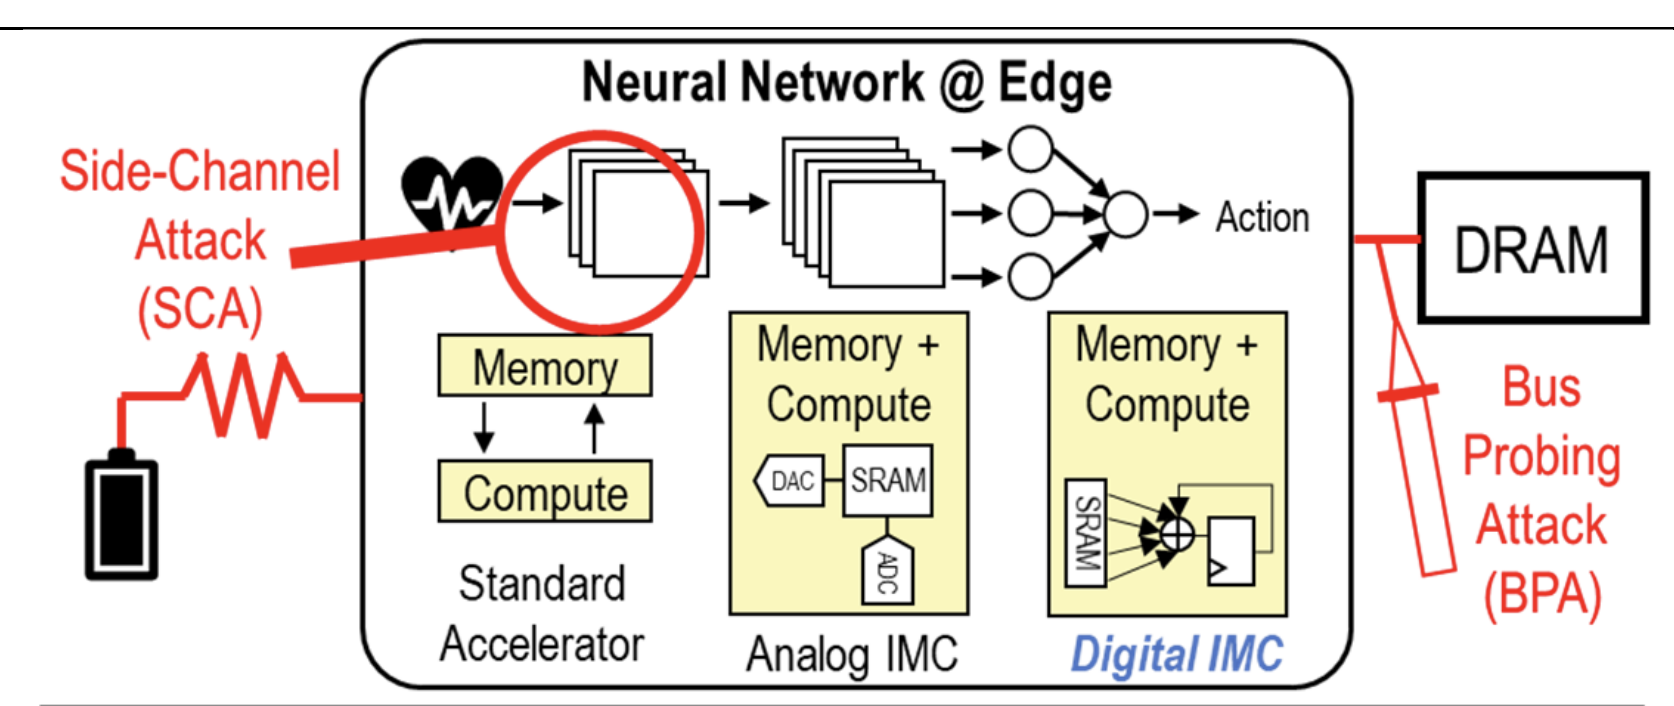
\includegraphics[width=0.5\linewidth]{sca_figure.png}
    \caption{Threat landscape for Neural Networks at the Edge, illustrating non-invasive Side-Channel Attacks (SCA) leveraging physical power signatures and semi-invasive Bus Probing Attacks (BPA) targeting external memory interfaces.}
    \label{fig:placeholder}
\end{figure}

\section{Methodology}
\subsection{Threat Model and Security Assumptions}
In alignment with standard hardware security evaluations, we assume a powerful adversary with local, physical access to the edge device. The attacker is capable of performing non-invasive Side-Channel Attacks (SCA), specifically monitoring the dynamic power consumption and electromagnetic (EM) emissions during neural network inference. Furthermore, we assume the adversary operates under Kerckhoffs's principle, possessing full knowledge of the implemented neural network architecture, masking algorithms, and the underlying DIMC hardware logic, lacking only the proprietary model weights. The primary objective of this architecture is to provide provable resistance against first-order attacks and ensure Probe-Isolating Non-Interference (PINI) for the internal datapath, strictly limiting any internal probe leakage to a single share index.

To achieve a balance between robust Side-Channel Attack (SCA) resistance and the area constraints of edge devices, this work proposes a hybrid security architecture, as illustrated in Fig. \ref{fig:dimc_core}. The methodology centers on the principle that mathematical linearity is domain-dependent, allowing for the strategic partitioning of operations between algorithmic masking and physical countermeasures.

\subsection{Masking Domains and Linearity Constraints}
Hardware masking relies on splitting a sensitive variable $x$ into independent shares to decorrelate the power consumption from the underlying data. We distinguish between two primary masking domains utilized in this architecture:

\begin{enumerate}
    \item \textbf{Boolean Masking:} A variable $x$ is represented by $n$ shares (where $n=3$ for this implementation) such that:
    \begin{equation}
    x = x_1 \oplus x_2 \oplus x_3
    \label{eq:boolean}
    \end{equation}
    This domain is highly efficient for bitwise XOR operations but incurs significant overhead for arithmetic operations.
    
    \item \textbf{Additive (Arithmetic) Masking:} A variable $x$ is represented as:
    \begin{equation}
    x = (A + B + \dots) \pmod{2^k}
    \label{eq:additive}
    \end{equation}
    While addition is linear in this domain, bitwise logic becomes non-linear and area-prohibitive.
\end{enumerate}

\begin{figure}[ht]
    \centering
    % Ensure this matches the uploaded filename in Overleaf!
    \includegraphics[width=0.85\columnwidth]{ti_and_gate.png} 
    \caption{Logic expansion of a single AND gate using a 3-share Threshold Implementation (TI). The requirement to compute nine distinct cross-products significantly increases the logic depth and area overhead compared to the unprotected baseline.}
    \label{fig:ti_and}
\end{figure}

The fundamental challenge in secure DIMC design is that standard \textbf{AND}-based multiplication is non-linear relative to the Boolean domain defined in (\ref{eq:boolean}). As illustrated in Fig. \ref{fig:ti_and}, protecting a single non-linear AND operation requires evaluating nine distinct cross-product terms to maintain the non-completeness property. Implementing these complex non-linear gadgets directly in hardware leads to a massive bloat in area overhead—often resulting in a core $12\times$ to $13\times$ the size of an unprotected baseline.

\subsection{Linearized IMC Multiplication via XNOR}
To alleviate the non-linearity tax, our methodology utilizes \textbf{XNOR-based bitwise multiplication} within the IMC macro (labeled as the DIMC Array in Fig. \ref{fig:dimc_core}). By restructuring the multiplication to be linear in the Boolean domain, we ensure that partial products can be computed and processed through a 3-share masked \textbf{Tree Adder} without inter-share communication. This approach satisfies the \textit{Non-completeness} property of Threshold Implementation (TI), preventing leakage even in the presence of hardware glitches, while significantly reducing the logic depth and area footprint compared to masked AND-gates. To compensate for the functional divergence from traditional arithmetic, an algorithmic offset correction is integrated into the near-memory post-processing unit. This refinement ensures the final results are mathematically equivalent to standard AND-based multiplication, maintaining inference accuracy while preserving the security benefits of the linearized datapath.

\subsection{Near-Memory Post-Computation Partitioning}
While the high-parallelism MAC operations are performed within the IMC macro, the non-linear layers—specifically \textbf{Batch Normalization}, \textbf{ReLU} and the \textbf{Multiplier Offset Correction} —are executed as post-computation in the Near-Memory Computing (NMC) unit. By partitioning the architecture this way, we avoid the prohibitive cost of implementing non-linear Boolean masking for the entire pipeline. To further mitigate the area bloat inherent in multi-share masking schemes, the NMC unit is architected to reuse the same hardware logic for both final multi-bit accumulation and Batch Normalization. This is achieved by pre-calculating the Batch Normalization layers into known coefficients, allowing the operation to be implemented as a simplified shift-and-add sequence rather than requiring complex, area-prohibitive multiplication and addition units. 



We aim to secure these specific near-memory bottlenecks using physical security measures, such as switched-capacitor logic, to decouple the digital switching activity from the $V_{DD}$ supply. This hybrid strategy of hardware reuse and localized physical countermeasures allows the system to support a full neural network inference flow while targeting an aggregate area overhead of only $5\times$ compared to the unprotected baseline.

\subsection{Side-Channel Evaluation Methodology}
To rigorously evaluate the security of the proposed DIMC core, we implemented an automated Side-Channel Analysis (SCA) verification flow. 
The evaluation methodology is based on the Test Vector Leakage Assessment (TVLA) using Welch's T-test, which provides a statistical measure of whether the device's power consumption is independent of the processed data. 

We utilize a "Fixed vs. Random" testing protocol, where the hardware is subjected to 60,000 trials. 
The power consumption traces are extracted via post-synthesis gate-level simulations using Synopsys PrimeTime PX to capture the dynamic switching activity at a 10ps resolution. 
The T-statistic is calculated at each time point according to equation 3.
\begin{equation}
t = \frac{\mu_{fixed} - \mu_{random}}{\sqrt{\frac{s_{fixed}^2}{N_{fixed}} + \frac{s_{random}^2}{N_{random}}}}
\end{equation}

Where $\mu_{fixed}$ and $\mu_{random}$ represent the mean power consumption of the fixed and random data sets, respectively; $s$ denotes the standard deviation; and $N$ represents the number of trials ($N=30,000$ per set). 
A T-statistic exceeding the threshold of $|t| > 4.5$ is defined as a failure, indicating a statistically significant leakage of sensitive information.

\subsection{Memory Array Integration}
A 6 transistor based SRAM memory array was also designed with a targeted 1GHz operating frequency using the same TSMC 28nm technology node. The read and write cycle performances of the are illustrated in \ref{fig:Read Cycle Delay} and \ref{fig:Write Cycle Delay} respectively. The critical path read cycle delay is measured from the decoder output to the SRAM and lastly the sense amplifier. The read cycle delay of the memory array is 310ps and the write cycle delay is 39.6ps in the TT corner. 

The entire memory array circuitry including the peripherals were tested across all process and temperature variation corners and was validated to operate at a frequency of 1GHz even for SS corner conforming to the original frequency target.
\begin{figure}
    \centering
    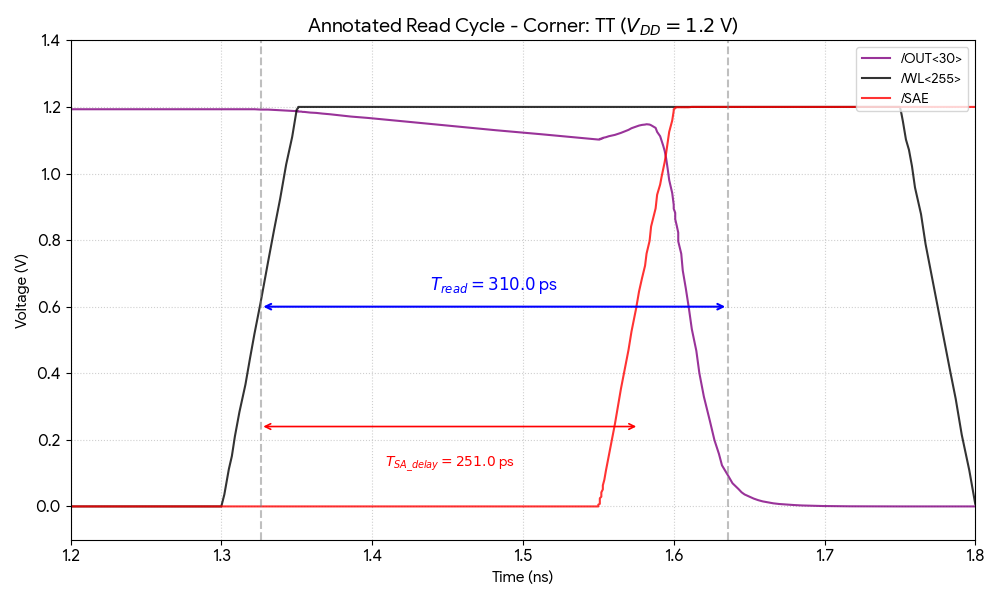
\includegraphics[width=0.5\linewidth]{read_cycle.png}
    \caption{Write Cycle graph of the memory array simulated with post layout load}
    \label{fig:Write Cycle Delay}
\end{figure}
\begin{figure}
        \centering
        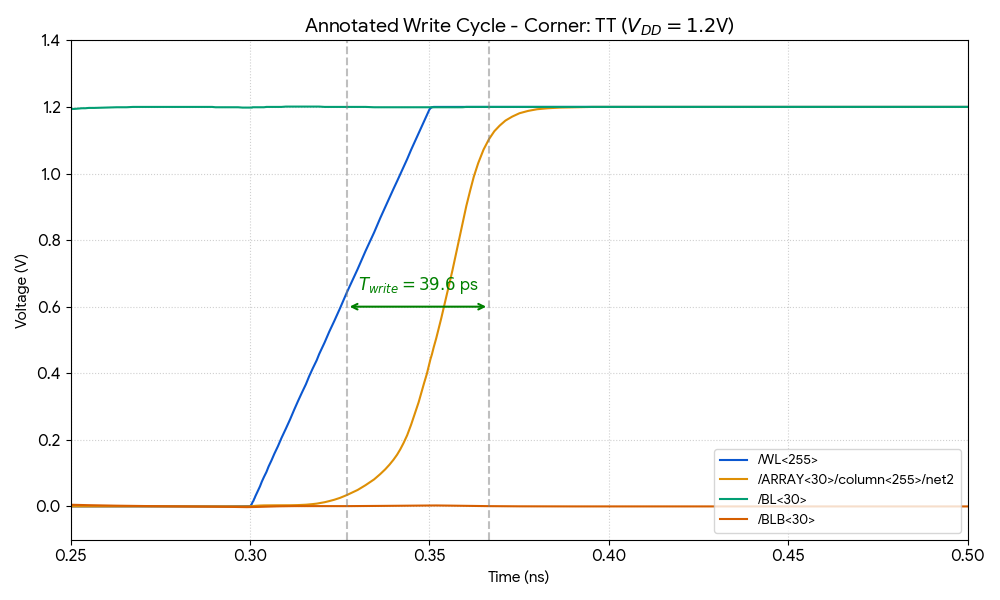
\includegraphics[width=0.5\linewidth]{write_cycle.png}
        \caption{Read Cycle graph of the memory array simulated with post layout load}
        \label{fig:Read Cycle Delay}
    \end{figure}
        

\begin{figure}[t]
    \centering
    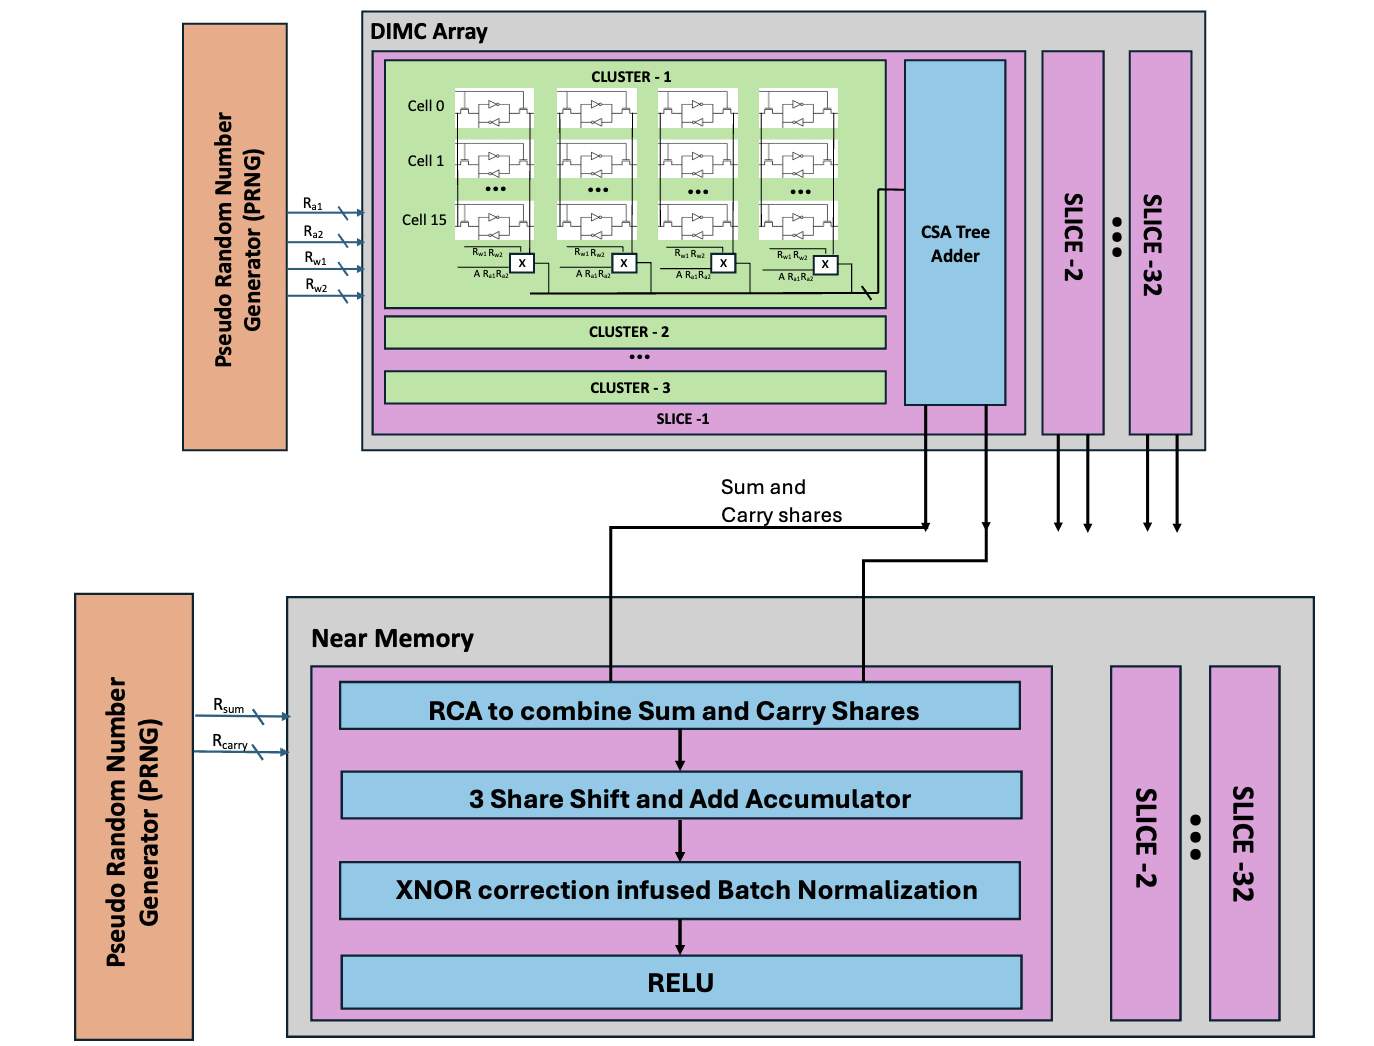
\includegraphics[width=1.0\columnwidth]{dimc_core.png}
    \caption{Architecture of the secure DIMC core featuring 3-share Boolean masking, CSA tree integration, and XNOR-correction infused Batch Normalization.}
    \label{fig:dimc_core}
\end{figure}


\section{Preliminary Results}

As this work represents an ongoing development effort, the results presented herein reflect the functional verification and initial hardware synthesis of the core architectural components prior to full-system integration.

\subsection{Algorithm-Level Verification}
The mathematical viability of the hybrid masking approach was validated through high-level software modeling. Specifically, the \textbf{XNOR offset correction} methodology was implemented and tested via a Python-based verification script. Simulations confirm that the statistical offsets introduced by substituting standard AND-based multipliers with linear XNOR logic can be fully compensated during the near-memory Batch Normalization phase, ensuring the inference accuracy is not degraded. The AND based multiplication results can be obtained from the XNOR based results as shown in equation 4.
\begin{equation}
X_{AND} = \frac{X_{NOR} - \text{Offset}}{2}
\end{equation}

Where the statistical offset for an $N$-input accumulation is derived from the summation of the input activations ($A$) and weights ($W$) shown in equation 5.

\begin{equation}
\text{Offset} = N - \left( \sum_{i=1}^{N} A_i + \sum_{i=1}^{N} W_i \right)
\end{equation}

This methodology ensures that the DIMC array remains purely linear for Boolean masking while allowing the PPU to reconstruct the non-linear MAC results required for downstream layers such as Batch Normalization and ReLU

\subsection{Area Analysis and Logic Overhead}
Synthesis results for the Carry Save Adder (CSA) tree variants, targeting the TSMC 28nm HPC+ process node, are summarized in Table \ref{tab:comp_synth_results}. 

The 3-share Boolean masking implementation utilizes 4,084 combinational cells, resulting in a total area of 3,063.56 $\mu m^2$. 
In contrast, the optimized Hybrid 2-share variant achieves a significant reduction in physical footprint, occupying only 935.00 $\mu m^2$. 
While the Hybrid design offers superior area efficiency, the subsequent side-channel analysis reveals a critical security-performance trade-off.

As detailed in Table \ref{tab:comp_synth_results}, the initial synthesis was targeted to a \textbf{TSMC 28nm HPC+} process node. The synthesis report confirms that the CSA tree is purely combinational, requiring 4,176 standard cells and occupying a total cell area of 3,063.56 $\mu\mathrm{m}^2$. This preliminary area extraction establishes the physical baseline for the masked IMC logic, verifying that the linear partial-product summation does not trigger the exponential gate explosion characteristic of masked AND-operations.

\begin{table}[h]
\renewcommand{\arraystretch}{1.3}
\caption{Comparative Synthesis Results: Hybrid 2-Share vs. 3-Share CSA Tree}
\label{tab:comp_synth_results}
\centering
\begin{tabular}{|l|c|c|}
\hline
\textbf{Parameter} & \textbf{Hybrid 2-Share CSA} & \textbf{3-Share CSA} \\
\hline
\hline
Technology Node & TSMC 28nm HPC+ & TSMC 28nm HPC+ \\
\hline
Combinational Cells & 1,602 & 4,084 \\
\hline
Buffer/Inverter Cells & 338 & 324 \\
\hline
\textbf{Total Cell Area} & \textbf{935.00 $\mu\mathrm{m}^2$} & \textbf{3063.56 $\mu\mathrm{m}^2$} \\
\hline
\end{tabular}
\end{table}


\subsection{Side-Channel Evaluation}
The empirical security of the proposed DIMC core was evaluated using an automated Side-Channel Analysis (SCA) verification flow. This methodology is centered on the Test Vector Leakage Assessment (TVLA) using Welch's T-test, which provides a statistical measure of whether the device's power consumption is independent of the processed data. We utilized a ``Fixed vs. Random'' testing protocol where the hardware was subjected to 60,000 trials to ensure statistical significance beyond preliminary noise floors. The power consumption traces were extracted via post-synthesis gate-level simulations using Synopsys PrimeTime PX to capture dynamic switching activity at a 10ps resolution. The T-statistic was calculated at each time point to determine if the magnitude $|t|$ exceeded the standard security threshold of 4.5.

The results of this 60,000-trial gauntlet, conducted on the design variants synthesized in TSMC 28nm HPC+, are illustrated in Fig. 6. The evaluation of the Hybrid 2-share baseline revealed a significant T-statistic failure, reaching a magnitude of $|t| \approx 10$ at the 5ns timestamp as shown in Fig. 6(a). This is starkly contrasted by the performance of the 3-share Boolean masking implementation, which successfully maintained a robust security floor with $|t| < 3$ throughout the entire 20ns clock period (Fig. 6(b)). Furthermore, the mean power signature overlay in Fig. 6(c) demonstrates near-perfect alignment between the Fixed and Random data sets. This symmetry confirms that the 3-share architecture effectively decorrelates internal switching activity to prevent first-order leakage, satisfying the requirements for secure edge AI deployment.


\begin{figure*}[t]
    \centering
    % Subfigure A: The Hybrid Leak
    \begin{subfigure}[b]{0.32\textwidth}
        \centering
        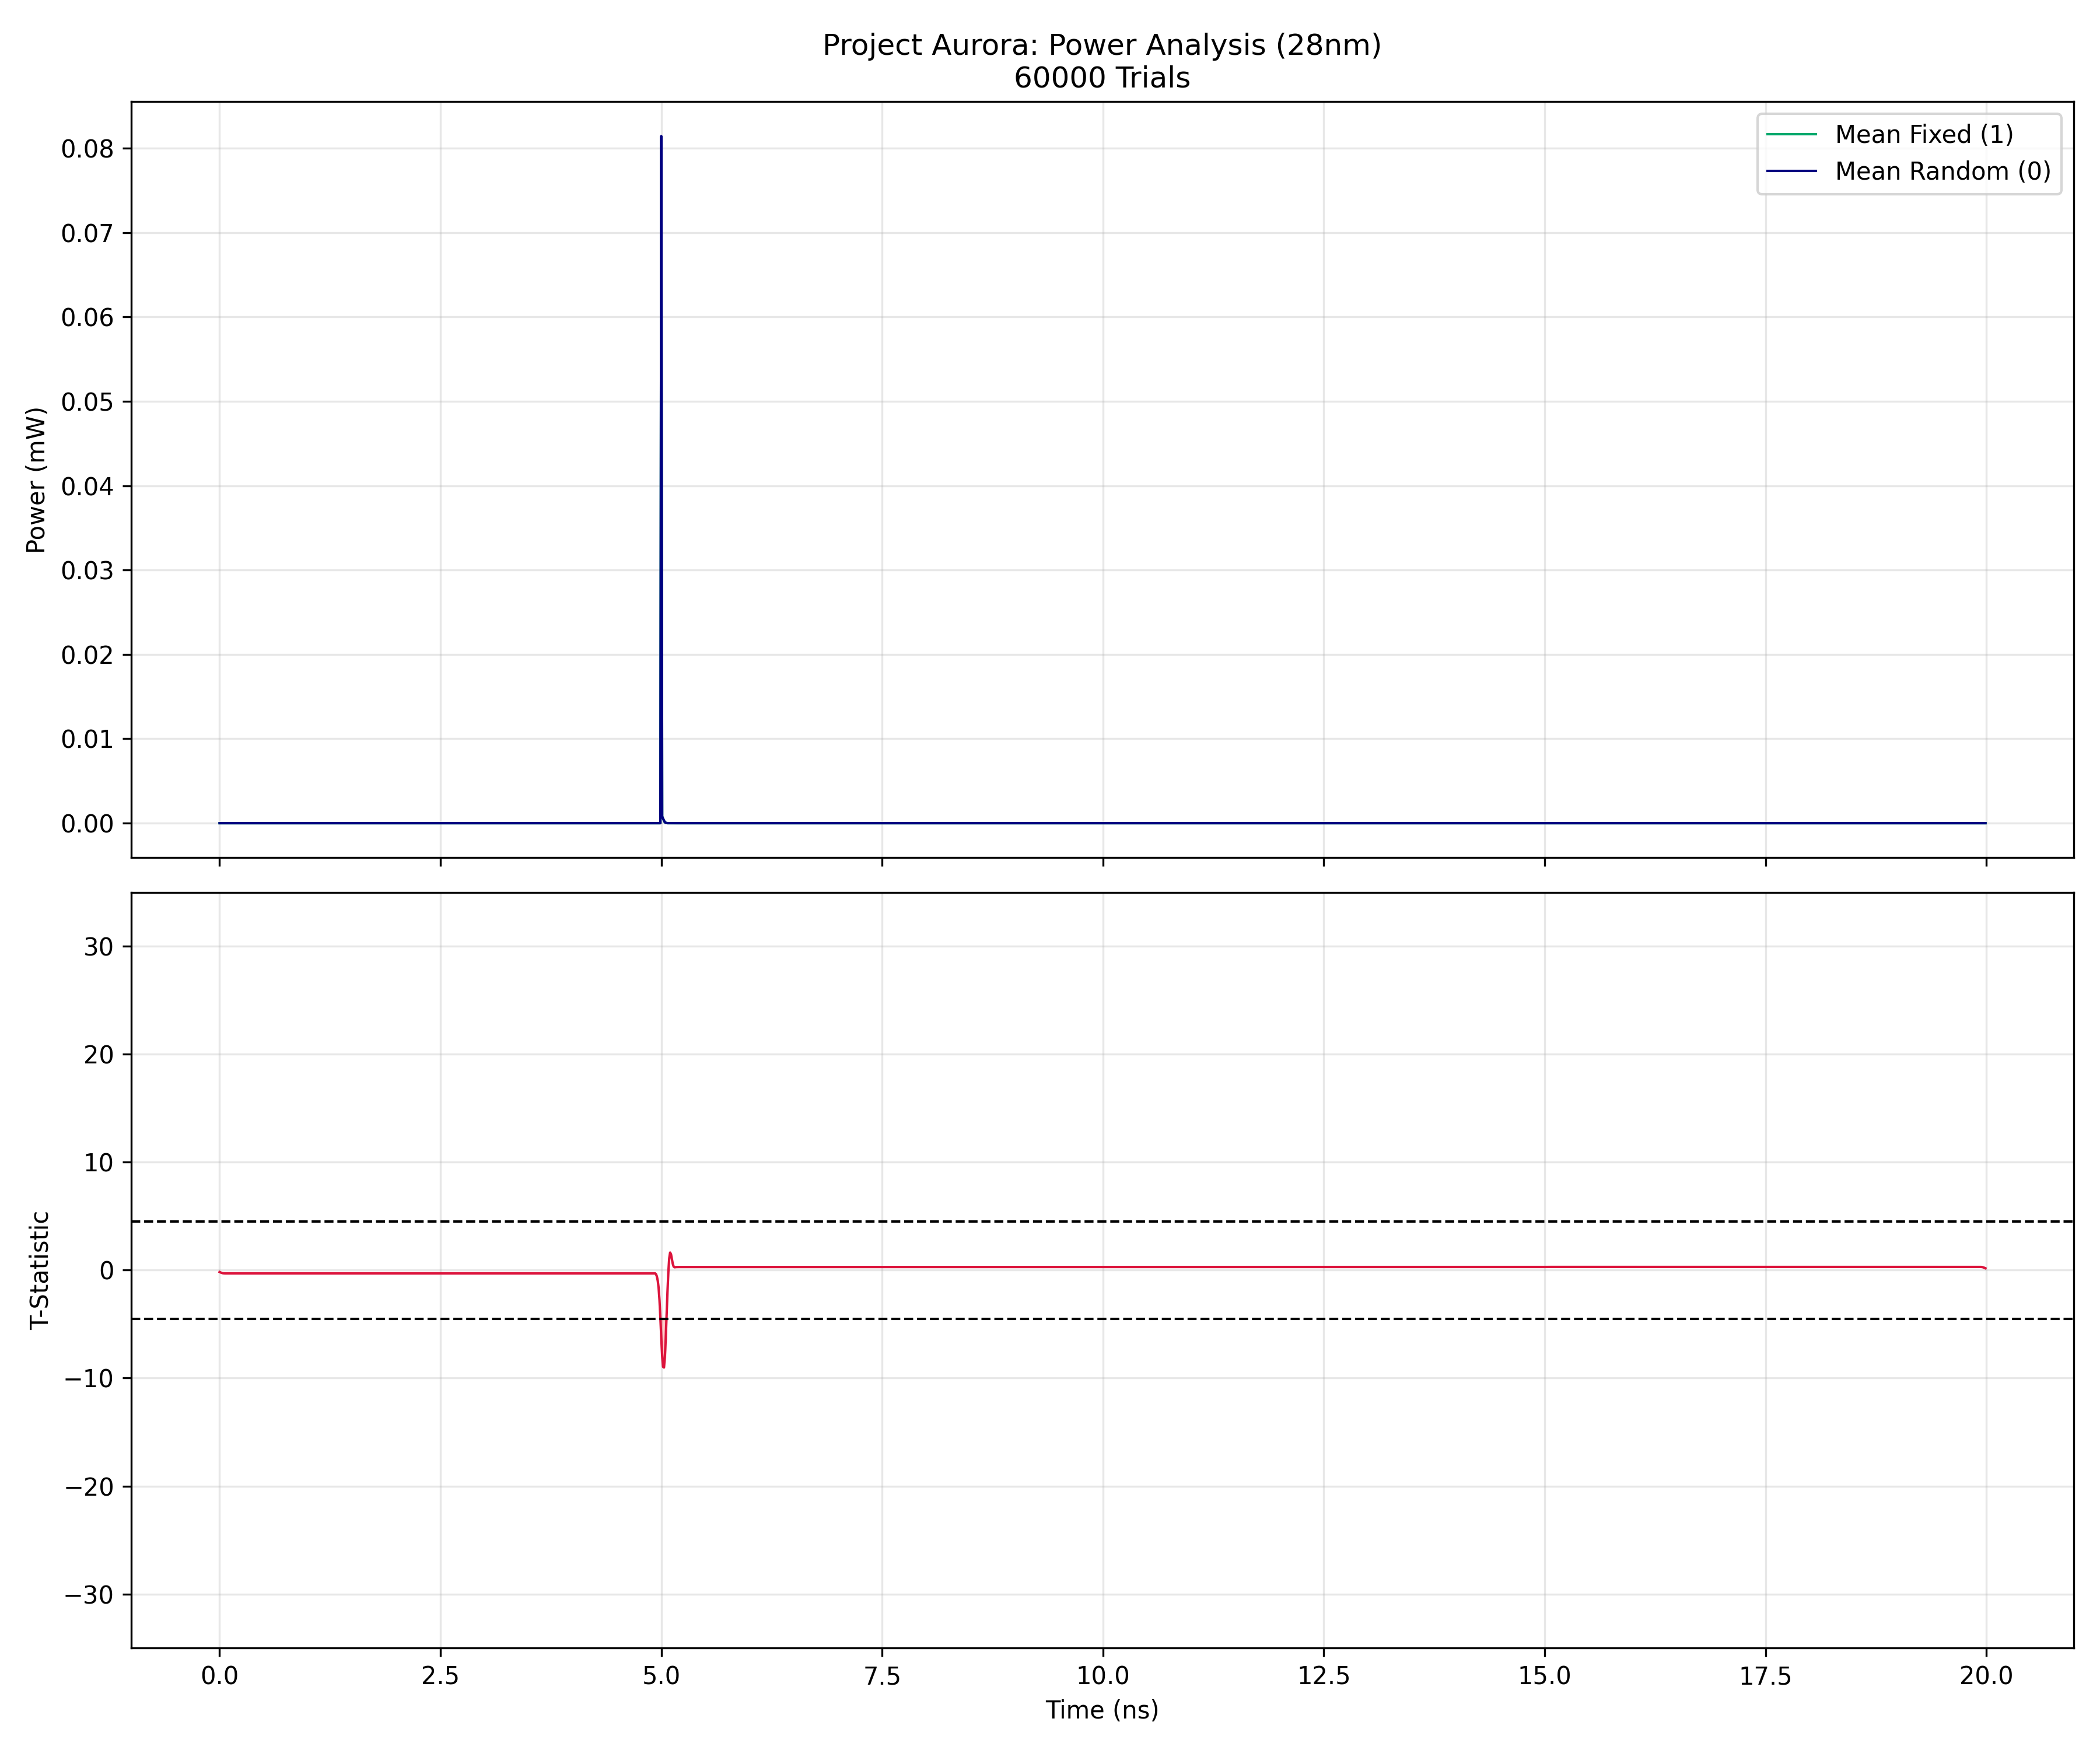
\includegraphics[width=\textwidth]{hybrid_60k.png}
        \caption{Hybrid 2-Share ($|T| \approx 10$)}
        \label{fig:hybrid_leak}
    \end{subfigure}
    \hfill
    % Subfigure B: The 3-Share Pass
    \begin{subfigure}[b]{0.32\textwidth}
        \centering
        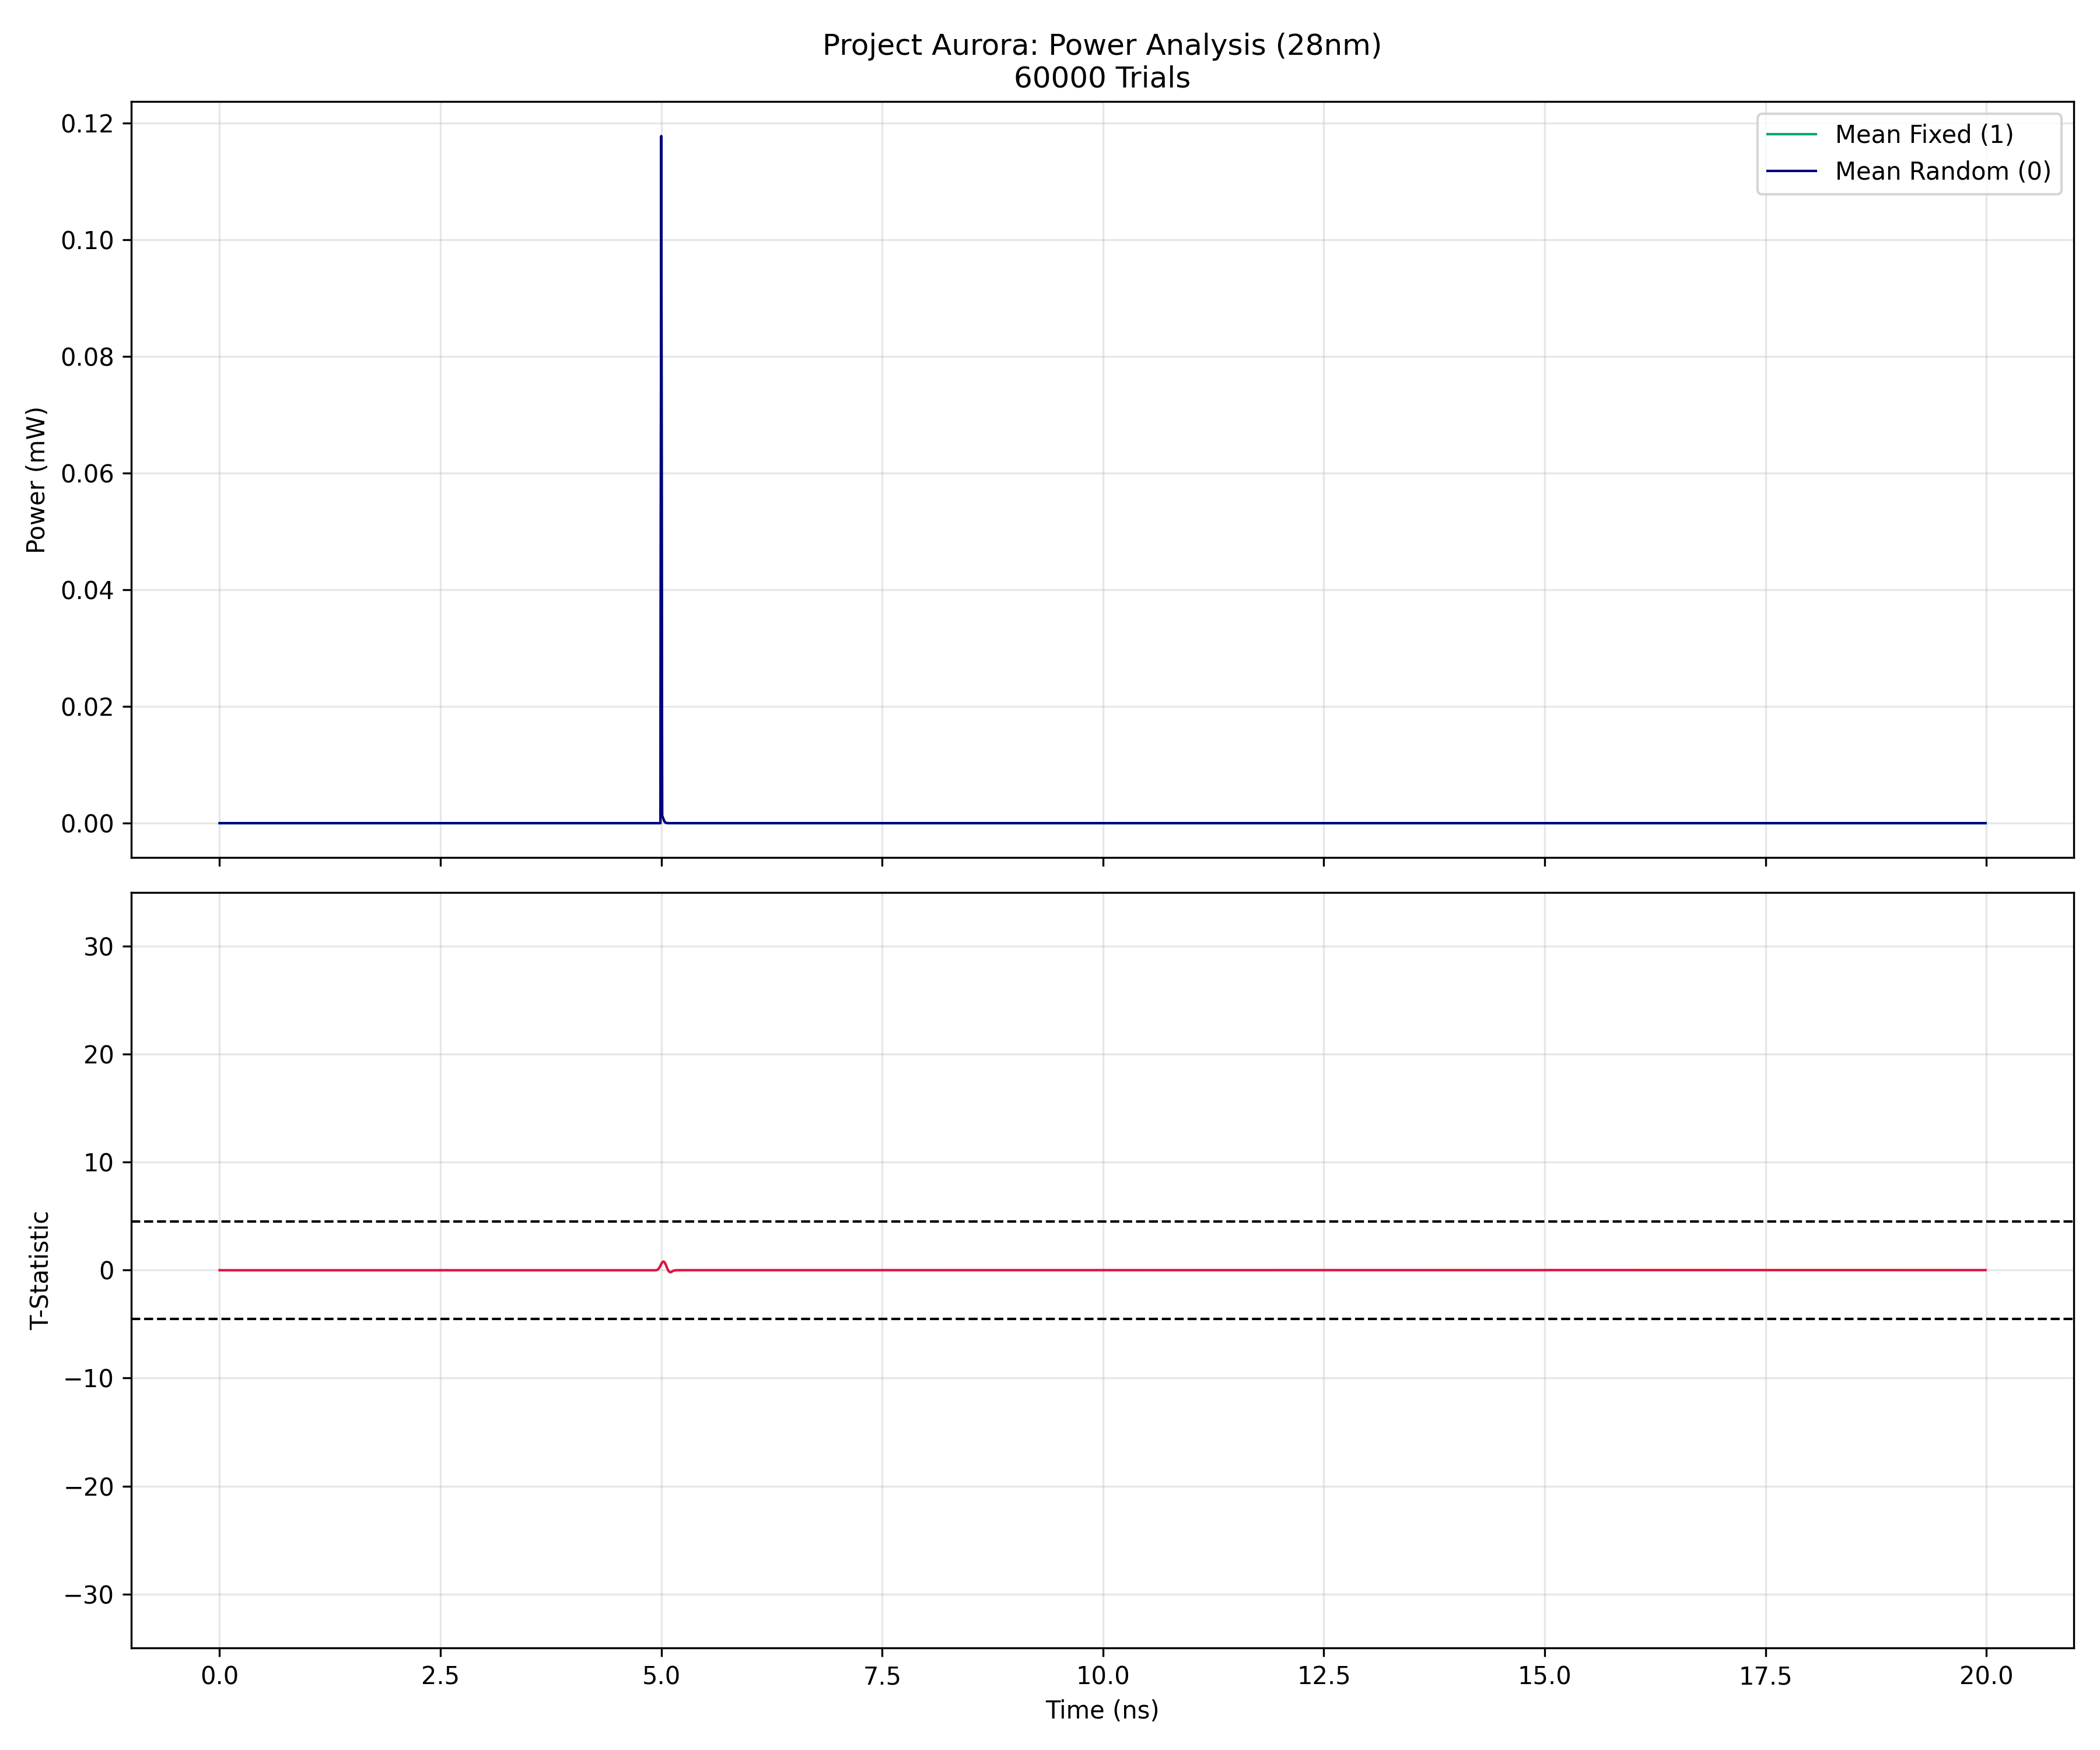
\includegraphics[width=\textwidth]{3share_60k.png}
        \caption{3-Share Robustness ($|T| < 3$)}
        \label{fig:three_share_pass}
    \end{subfigure}
    \hfill
    % Subfigure C: The Power Overlay
    \begin{subfigure}[b]{0.32\textwidth}
        \centering
        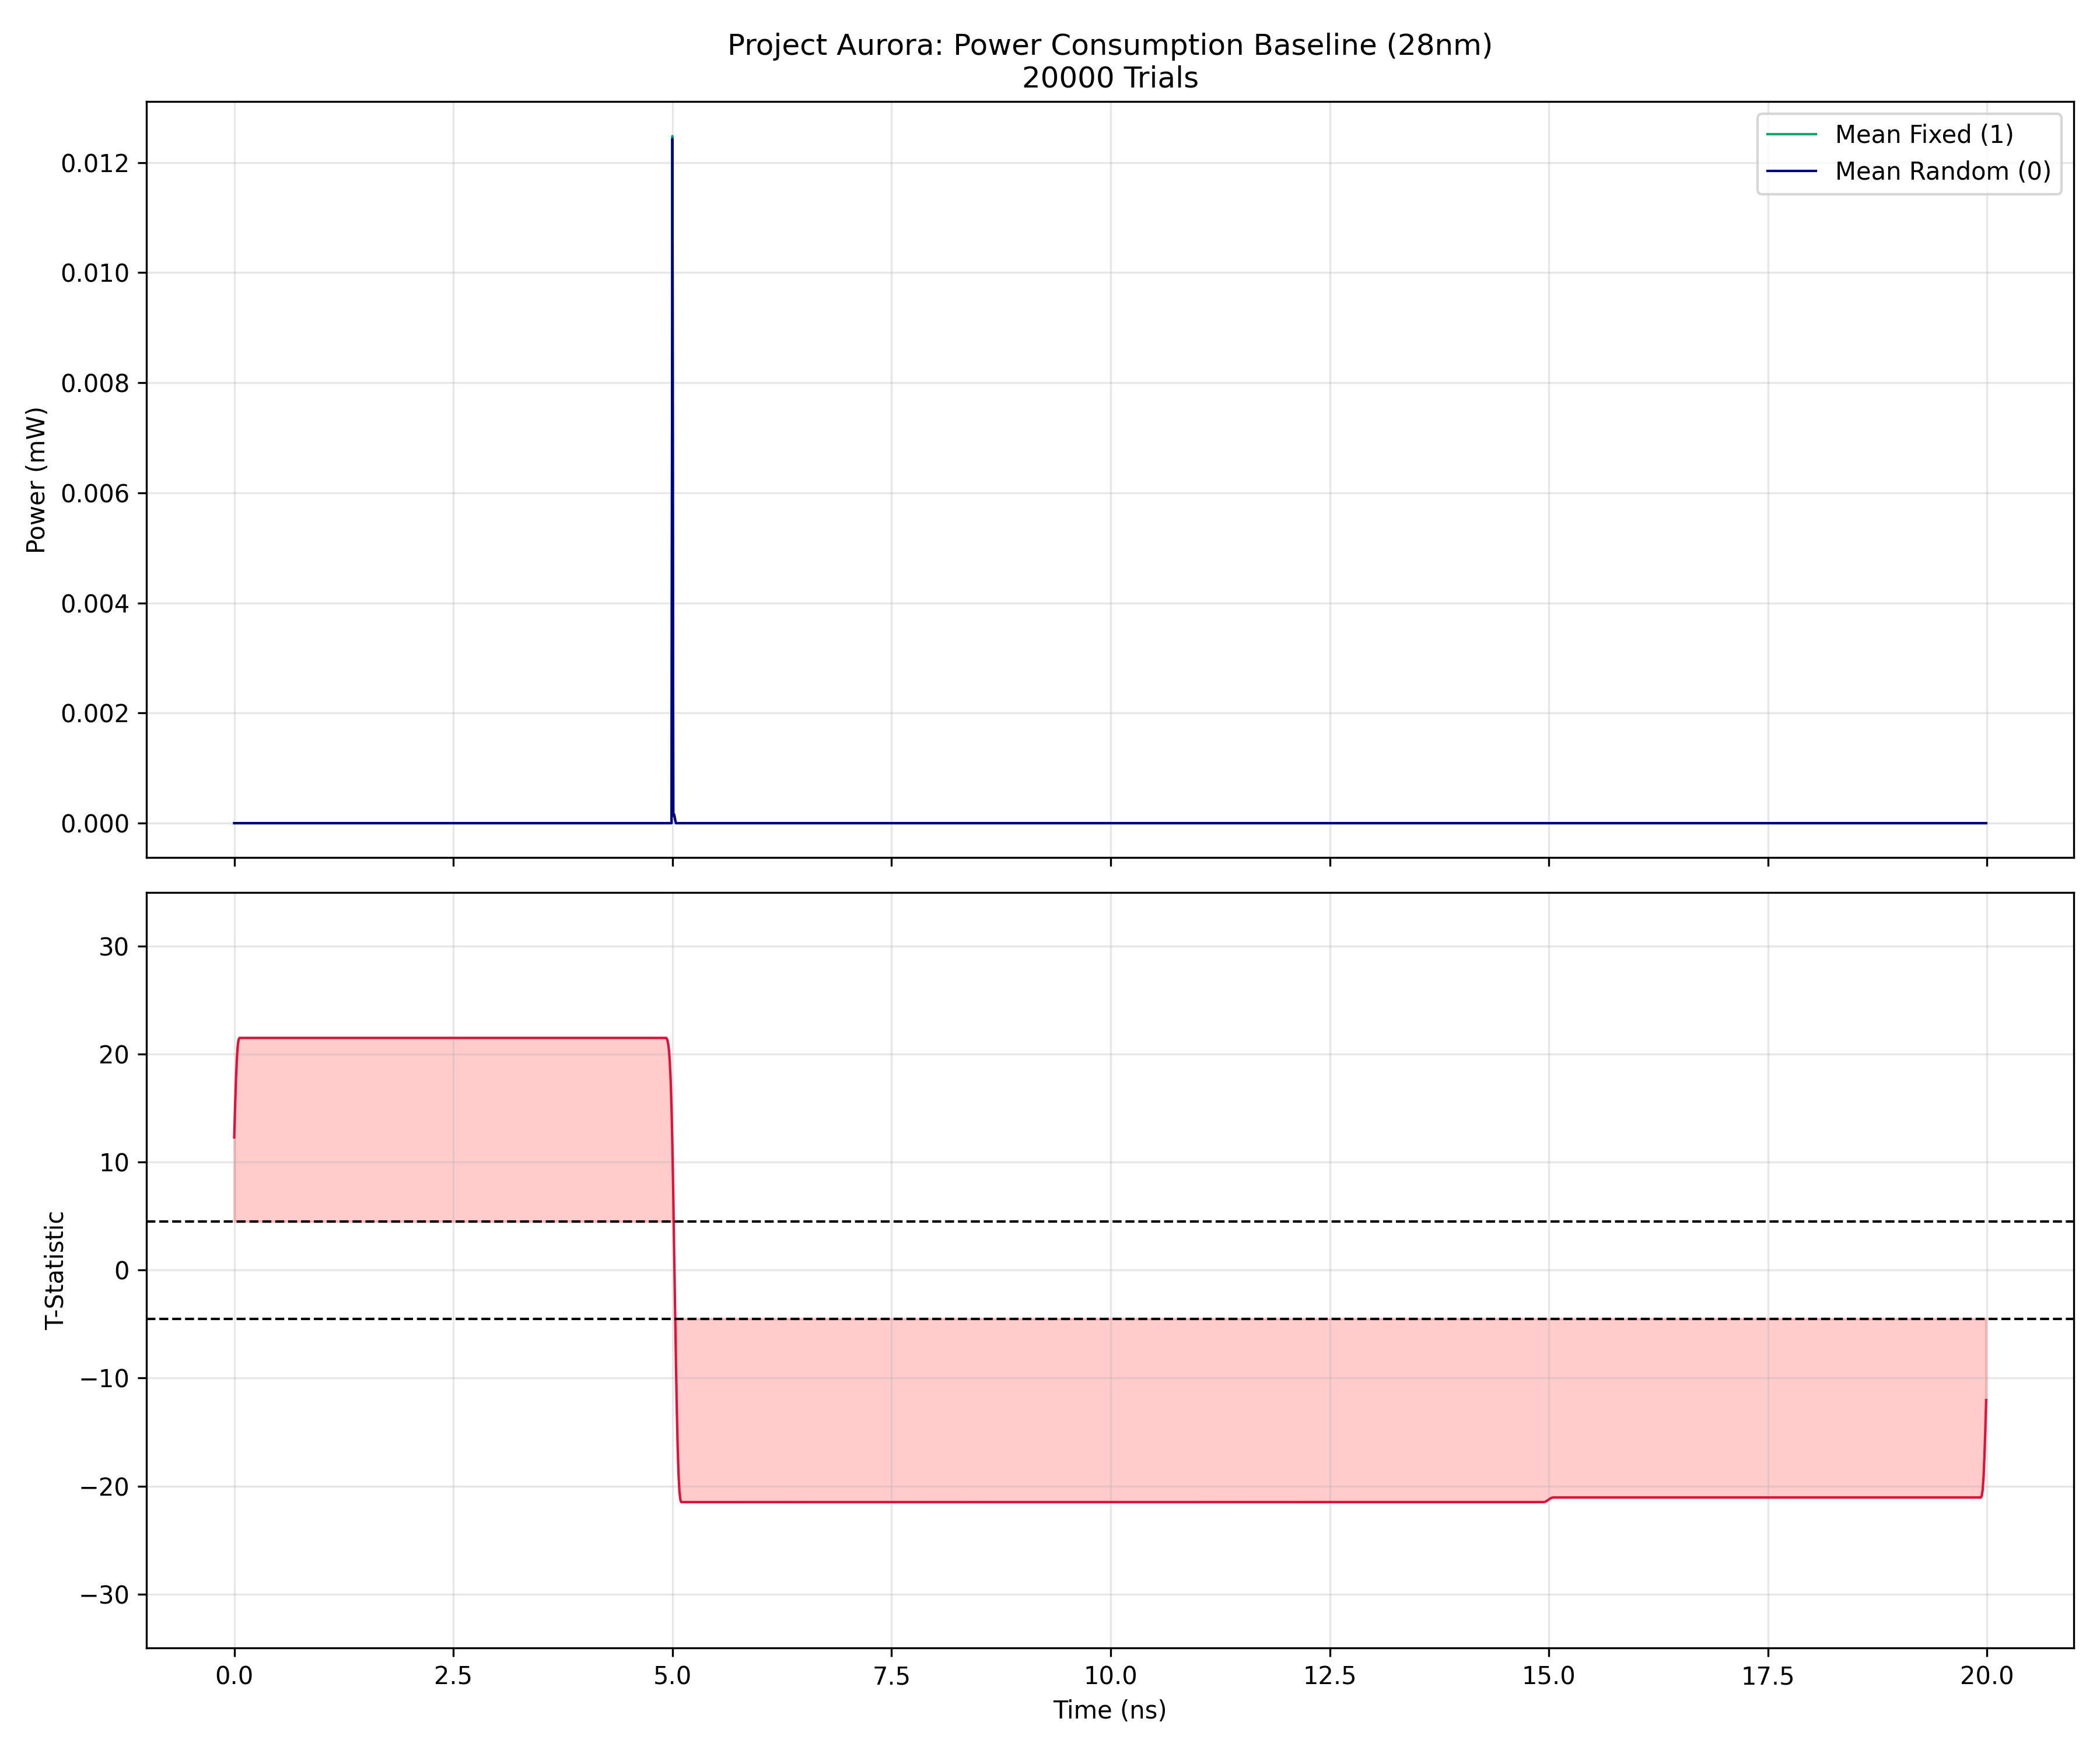
\includegraphics[width=\textwidth]{aurora_tvla_final.png}
        \caption{Mean Power Signature Overlay}
        \label{fig:power_overlay}
    \end{subfigure}
    \caption{Empirical Side-Channel Analysis for Project Aurora at 28nm. (a) Significant first-order leakage identified at the 5ns clock edge in the Hybrid implementation. (b) Successful suppression of data-dependent power signatures using 3-share Boolean masking at 60,000 trials. (c) Comparison of the mean power signatures for Fixed vs. Random trial sets.}
    \label{fig:sca_results}
\end{figure*}
\section{Discussion and Ongoing Work}

The preliminary synthesis of the Carry Save Adder (CSA) tree validates the primary hypothesis of this architecture: linearizing In-Memory Computing (IMC) arithmetic via XNOR-based logic successfully bypasses the exponential area bloat characteristic of traditional masked multipliers. However, evaluating these results from a physical layout perspective reveals a critical architectural constraint regarding the integration of Boolean masking. Extending a pure 3-share scheme throughout the entire multi-bit accumulation phase would introduce severe pitch-matching complications with the memory array columns, potentially compromising macro density. Consequently, a strict architectural boundary must be maintained, where Boolean partial-product generation is prioritized for its high efficiency.

The empirical results from the 60,000-trial TVLA gauntlet further reinforce the necessity of this design partitioning. While the Hybrid 2-share variant offers a minimized physical footprint, its failure at the 5ns clock edge confirms that first-order masking alone is insufficient to suppress data-dependent glitches and physical imbalances at the 28nm node. By contrast, the 3-share implementation satisfies the Non-completeness property of Threshold Implementations (TI), ensuring the secret state remains statistically hidden even at high sample counts. Although this implementation utilizes 4,084 combinational cells, the aggregate area overhead of approximately $4\times$ remains well below the initial $5\times$ target projected for the secure core.

Moving forward, the research will transition from global logic verification to localized physical optimization. The immediate roadmap for the Summer 2026 term involves a three-tier development phase focused on node-level leakage isolation, surgical physical security, and RTL integration. First, we will advance the automated verification flow to perform net-level power analysis using PrimeTime PX to identify the precise gates within the carry-propagation chain responsible for the 5ns leakage. Second, rather than utilizing globally redundant masking logic, we will apply ``surgical'' patches to the identified leaky nodes. This includes implementing targeted physical countermeasures—such as signal shielding and capacitive decoupling within the 28nm layout—to further optimize the area-security Pareto front. 

Finally, the Near-Memory Post-Processing Unit is currently being developed at the RTL level to integrate multi-bit accumulation, algorithmic XNOR offset correction, and Batch Normalization into a single pipeline. To maintain the strict area budget, the security of this unit will rely on physical hardware countermeasures, such as switched-capacitor logic, to decouple digital switching activity from the primary $V_{DD}$ supply The ultimate objective is to execute standardized workloads, such as CIFAR-10, through comprehensive Correlation Power Analysis (CPA) simulations to empirically demonstrate the core's robust resistance to side-channel attacks while maintaining the high efficiency required for next-generation edge AI deployment.




% needed in second column of first page if using \IEEEpubid
%\IEEEpubidadjcol




% An example of a floating figure using the graphicx package.
% Note that \label must occur AFTER (or within) \caption.
% For figures, \caption should occur after the \includegraphics.
% Note that IEEEtran v1.7 and later has special internal code that
% is designed to preserve the operation of \label within \caption
% even when the captionsoff option is in effect. However, because
% of issues like this, it may be the safest practice to put all your
% \label just after \caption rather than within \caption{}.
%
% Reminder: the "draftcls" or "draftclsnofoot", not "draft", class
% option should be used if it is desired that the figures are to be
% displayed while in draft mode.
%
%\begin{figure}[!t]
%\centering
%\includegraphics[width=2.5in]{myfigure}
% where an .eps filename suffix will be assumed under latex, 
% and a .pdf suffix will be assumed for pdflatex; or what has been declared
% via \DeclareGraphicsExtensions.
%\caption{Simulation results for the network.}
%\label{fig_sim}
%\end{figure}

% Note that the IEEE typically puts floats only at the top, even when this
% results in a large percentage of a column being occupied by floats.


% An example of a double column floating figure using two subfigures.
% (The subfig.sty package must be loaded for this to work.)
% The subfigure \label commands are set within each subfloat command,
% and the \label for the overall figure must come after \caption.
% \hfil is used as a separator to get equal spacing.
% Watch out that the combined width of all the subfigures on a 
% line do not exceed the text width or a line break will occur.
%
%\begin{figure*}[!t]
%\centering
%\subfloat[Case I]{\includegraphics[width=2.5in]{box}%
%\label{fig_first_case}}
%\hfil
%\subfloat[Case II]{\includegraphics[width=2.5in]{box}%
%\label{fig_second_case}}
%\caption{Simulation results for the network.}
%\label{fig_sim}
%\end{figure*}
%
% Note that often IEEE papers with subfigures do not employ subfigure
% captions (using the optional argument to \subfloat[]), but instead will
% reference/describe all of them (a), (b), etc., within the main caption.
% Be aware that for subfig.sty to generate the (a), (b), etc., subfigure
% labels, the optional argument to \subfloat must be present. If a
% subcaption is not desired, just leave its contents blank,
% e.g., \subfloat[].


% An example of a floating table. Note that, for IEEE style tables, the
% \caption command should come BEFORE the table and, given that table
% captions serve much like titles, are usually capitalized except for words
% such as a, an, and, as, at, but, by, for, in, nor, of, on, or, the, to
% and up, which are usually not capitalized unless they are the first or
% last word of the caption. Table text will default to \footnotesize as
% the IEEE normally uses this smaller font for tables.
% The \label must come after \caption as always.
%
%\begin{table}[!t]
%% increase table row spacing, adjust to taste
%\renewcommand{\arraystretch}{1.3}
% if using array.sty, it might be a good idea to tweak the value of
% \extrarowheight as needed to properly center the text within the cells
%\caption{An Example of a Table}
%\label{table_example}
%\centering
%% Some packages, such as MDW tools, offer better commands for making tables
%% than the plain LaTeX2e tabular which is used here.
%\begin{tabular}{|c||c|}
%\hline
%One & Two\\
%\hline
%Three & Four\\
%\hline
%\end{tabular}
%\end{table}


% Note that the IEEE does not put floats in the very first column
% - or typically anywhere on the first page for that matter. Also,
% in-text middle ("here") positioning is typically not used, but it
% is allowed and encouraged for Computer Society conferences (but
% not Computer Society journals). Most IEEE journals/conferences use
% top floats exclusively. 
% Note that, LaTeX2e, unlike IEEE journals/conferences, places
% footnotes above bottom floats. This can be corrected via the
% \fnbelowfloat command of the stfloats package.







% if have a single appendix:
%\appendix[Proof of the Zonklar Equations]
% or
%\appendix  % for no appendix heading
% do not use \section anymore after \appendix, only \section*
% is possibly needed

% use appendices with more than one appendix
% then use \section to start each appendix
% you must declare a \section before using any
% \subsection or using \label (\appendices by itself
% starts a section numbered zero.)
%




% you can choose not to have a title for an appendix
% if you want by leaving the argument blank



% use section* for acknowledgment
\section*{Acknowledgment}
The authors would like to thank Professor Kaiyuan Yang and the Secure and Intelligent Micro-Systems (SIMS) Lab, as well as the Department of Electrical and Computer Engineering at Rice University, for their ongoing guidance and support.

% Can use something like this to put references on a page
% by themselves when using endfloat and the captionsoff option.
\ifCLASSOPTIONcaptionsoff
  \newpage
\fi

\section*{CRediT Author Statement}
\textbf{Ajay Sabareesh Balamurugan:} Conceptualization, Methodology, Software, Hardware, Validation, Formal Analysis, Investigation, Writing - Original Draft, Writing - Review \& Editing.


% trigger a \newpage just before the given reference
% number - used to balance the columns on the last page
% adjust value as needed - may need to be readjusted if
% the document is modified later
%\IEEEtriggeratref{8}
% The "triggered" command can be changed if desired:
%\IEEEtriggercmd{\enlargethispage{-5in}}

% references section

% can use a bibliography generated by BibTeX as a .bbl file
% BibTeX documentation can be easily obtained at:
% http://mirror.ctan.org/biblio/bibtex/contrib/doc/
% The IEEEtran BibTeX style support page is at:
% http://www.michaelshell.org/tex/ieeetran/bibtex/
%\bibliographystyle{IEEEtran}
% argument is your BibTeX string definitions and bibliography database(s)
%\bibliography{IEEEabrv,../bib/paper}
%
% <OR> manually copy in the resultant .bbl file
% set second argument of \begin to the number of references
% (used to reserve space for the reference number labels box)
\begin{thebibliography}{1}

\bibitem{ashok2024}
M. Ashok, S. Maji, X. Zhang, J. Cohn, and A. P. Chandrakasan, ``A Secure Digital In-Memory Compute (IMC) Macro with Protections for Side-Channel and Bus Probing Attacks,'' in \emph{Proc. IEEE CICC}, 2024, pp. 1--2.

\bibitem{schneider2015}
T. Schneider, A. Moradi, and T. G\"{u}neysu, ``Arithmetic Addition over Boolean Masking,'' in \emph{Proc. ACNS}, Springer, 2015.

\bibitem{wang2022}
D. Wang \emph{et al.}, ``DIMC: 2219TOPS/W 2569F$^2$/b digital in-memory computing macro in 28nm based on approximate arithmetic hardware,'' in \emph{Proc. IEEE ISSCC}, 2022.

\bibitem{maji2022}
S. Maji \emph{et al.}, ``A threshold implementation-based neural network accelerator with power and electromagnetic side-channel countermeasures,'' \emph{IEEE J. Solid-State Circuits}, vol. 58, no. 1, pp. 141--154, 2022.

\bibitem{goubin2001}
L. Goubin, ``A sound method for switching between boolean and arithmetic masking,'' in \emph{Proc. CHES}, Springer, 2001.

\bibitem{sasdrich2020}
P. Sasdrich, B. Bilgin, M. Hutter, and M. E. Marson, ``Low-latency hardware masking with application to AES,'' \emph{IACR Trans. Cryptogr. Hardw. Embed. Syst.}, vol. 2020, no. 2, pp. 300--326, 2020.

\bibitem{kumar2023}
S.~V.~D.~Kumar \emph{et al.}, ``Low-cost first-order secure Boolean masking in glitchy hardware,'' in \emph{Proc. DATE}, 2023.

\bibitem{bepary2024}
M. K. Bepary \emph{et al.}, ``Prescan: A comprehensive review of pre-silicon physical side-channel vulnerability assessment methodologies,'' \emph{Chips}, vol. 3, no. 4, pp. 311--333, 2024.

\bibitem{woudenberg2023}
J. Van Woudenberg \emph{et al.}, ``Pre-silicon side channel and fault analysis,'' in \emph{Proc. IEEE/ACM DAC}, 2023.

\bibitem{pundir2022}
N. Pundir, N. Selvakkumaran, A. S. Sadi, and F. Farahmandi, ``Power side-channel leakage assessment framework at register-transfer level,'' \emph{IEEE Trans. Very Large Scale Integr. (VLSI) Syst.}, vol. 30, no. 9, pp. 1207--1218, 2022.

\bibitem{bokharaie2022}
V. S. Bokharaie and A. Jahanian, ``Power side-channel leakage assessment and locating the exact sources of leakage at the early stages of ASIC design process,'' \emph{J. Supercomput.}, vol. 78, no. 2, pp. 2219--2244, 2022.

\end{thebibliography}
% biography section
% 
% If you have an EPS/PDF photo (graphicx package needed) extra braces are
% needed around the contents of the optional argument to biography to prevent
% the LaTeX parser from getting confused when it sees the complicated
% \includegraphics command within an optional argument. (You could create
% your own custom macro containing the \includegraphics command to make things
% simpler here.)
%\begin{IEEEbiography}[{\includegraphics[width=1in,height=1.25in,clip,keepaspectratio]{mshell}}]{Michael Shell}
% or if you just want to reserve a space for a photo:

% if you will not have a photo at all:


% insert where needed to balance the two columns on the last page with
% biographies
%\newpage



% You can push biographies down or up by placing
% a \vfill before or after them. The appropriate
% use of \vfill depends on what kind of text is
% on the last page and whether or not the columns
% are being equalized.

%\vfill

% Can be used to pull up biographies so that the bottom of the last one
% is flush with the other column.
%\enlargethispage{-5in}



% that's all folks
\end{document}


